\documentclass{article}
\usepackage[utf8]{inputenc}
\usepackage[T1]{fontenc}
\usepackage[french]{babel}
\usepackage{textcomp}
\usepackage{amsmath,amssymb,amsthm}
\usepackage{lmodern}
\usepackage[a4paper]{geometry}
\usepackage{graphicx}
\usepackage{xcolor}
\usepackage{multicol}
\usepackage{microtype}
\usepackage{pdfpages}
\usepackage{listings}
\usepackage{color}


\usepackage{hyperref}
\hypersetup{pdfstartview=XYZ}
 

\usepackage{fancyhdr}
\pagestyle{fancy}
\renewcommand\headrulewidth{0.4pt}
\fancyhead[L]{Le Cesne Benjamin - Tardy Luca}
\fancyhead[R]{Prep'ISIMA / L2 INFO}
\renewcommand\footrulewidth{0.4pt}
\fancyfoot[C]{
\textbf{Page \thepage/10}}
\fancyfoot[L]{\textit{Projet - Prep'ISIMA}}
\fancyfoot[R]{\today}

\newcommand{\variable}[1]{\texttt{#1}}
\newcommand{\code}[1]{\lstinputlisting{#1}}


\definecolor{darkWhite}{rgb}{0.92,0.92,0.92}

\lstset{frame=single,
  language=C,
  showstringspaces=false,
  columns=flexible,
  backgroundcolor=\color{darkWhite},
  basicstyle={\small\ttfamily},
  numbers=left,
  numberstyle=\tiny\color{black},
  framexleftmargin=20pt,
  framexrightmargin=20pt,
  keywordstyle=\color{blue},
  commentstyle=\color{red},
  stringstyle=\color{violet},
  breaklines=true,
  breakatwhitespace=true,
  tabsize=2,
  literate=%
  {à}{{\`a }}1
  {é}{{\'e}}1
  {è}{{\`e}}1
  {ê}{{\^e}}1
  {ù}{{\`u}}1
  {î}{{\^i}}1
}


\begin {document}
\hfill
\hfill
\hfill
\begin{center}
  \large{PROJET EULER}

  Problème 117
\end{center}
\tableofcontents
\newpage
\part {Résolution du problème}
\section {Présentation}

Dans ce problème, il faut trouver combien il y a de possibilités pour remplir 50 cases avec des rectangles de longueurs 2, 3 et 4 cases, sachant que des cases peuvent rester vides et que l'ordre compte. Par exemple, il y a 15 manières de remplir 5 cases :
\bigbreak
\begin{center}
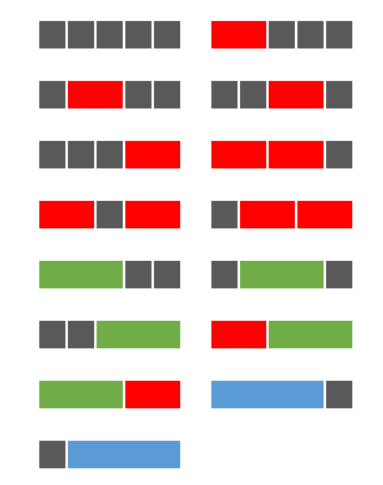
\includegraphics[scale = 0.5]{Images/presentation.png}
\end{center}
\bigbreak

\section{Méthodes de réflexion}

\subsection{Première méthode (méthode récursive)}

\subsubsection{Algorithme de principe}
\lstinputlisting[language=bash]{Algo_de_principe/problem117_1_principe.txt}

\subsubsection{Développement}
Dans cette méthode récursive, nous considérons que pour remplir les 50 cases il faut déjà commencer par choisir comment remplir la première case. Il y a 4 réponses possibles à cette question : soit on ne la remplit pas, soit on pose un rectangle de 2 cases, soit de 3 cases ou soit de 4 cases. Dans le premier cas, il ne restera plus que 49 cases à remplir. Dans le deuxième cas, il n'en restera que 48, 47 dans le troisième et 46 dans le dernier. C'est pourquoi nous appelons la même fonction de façon récursive pour calculer le nombre de possibilités de remplir 49, 48, 47 et 46 cases. Ensuite on répète ce processus d'appel récursif sur les 4 précédents jusqu'à trouver un cas d'arrêt. Les cas d'arrêts sont au nombre de 4 avec cette méthode. En effet, on connaît gràce à l'exemple donné précédemment, le nombre de possibilités pour remplir 5 cases, donc 5 est un cas d'arrêt et on retourne 15 dans ce cas-là. Mais il est possible que l'on n'appelle jamais la fonction avec n = 5. En effet, lorsque n = 6, on appelle $recursive(5)$, $recursive(4)$, $recursive(3)$ et $recursive(2)$. Ainsi, 4, 3 et 2 sont des cas d'arrêts également.

Ceci correspond ainsi à une modélisation de la suite de Tetranacci, une dérivé de la suite de Fibonacci. En effet, si on appelle $F$ la suite de Fibonacci, on sait que $F(n) = F(n-1) + F(n-2)$. Ici, on remarque que $recursive(n) = recursive(n-1) + recursive(n-2) + recursive(n-3) + recursive(n-4)$. Ceci correspond à une suite où chaque terme est la somme des 4 précédents, la suite de tetranacci. Malheureusement, cette méthode est beaucoup trop longue, comme pour Fibonacci. En prenant 50 comme entrée, elle doit faire un nombre incalculable d'appels récursifs. Il faut donc la modifier pour ne plus faire appels à la fonction plusieurs fois avec la même entrée. En effet, ici, on appelle plusieurs fois la même fonction avec le même argument. Par exemple, en partant de 50, on l'appelle avec 49, 48, 47 et 46. Mais avec 49, on l'appelle encore avec 48, 47 et 46. Ceci n'est que le début, à la fin, le programme va appeler cette fonction avec 6 un très grand nombre de fois. Il faut donc stocker le résultat de chaque appel pour ne plus avoir à le calculer.
\subsection{Seconde méthode (méthode tetranacci)}

\subsubsection{Algorithme de principe}
\lstinputlisting[language=bash]{Algo_de_principe/problem117_2_principe.txt}

\subsubsection{Développement}
Ici, on remarque que la suite de Tetranacci (que l'on appelera $T$) commence, comme Fibonacci, à 0. Ainsi, $T(0) = 1, T(1) = T(0), T(2) = T(0) + T(1) et T(3) = T(0) + T(1) + T(2)$. On sait que chaque terme est la somme des 4 précédents. Il faut donc stocker ces 4 termes pour ne pas avoir à les recalculer. On stocke donc dans une liste 4 valeurs. A l'initialisation, il ne doit y avoir que $T(0)$. Or, pour calculer $T(1)$, on doit avoir accès à 4 valeurs pour pouvoir calculer une somme. C'est pourquoi on initialise cette liste à $[0,0,0,T(0)]$. Ensuite, tant que nous n'avons pas $n+3$ valeurs dans la liste, on y ajoute le prochain terme en faisant la somme des 4 derniers termes. $T(n)$ sera le $n+3^{ème}$ terme puisque les 3 premiers ne font pas à proprement parler de la suite. Ainsi, on calcule $T(n)$ très rapidement, en ne calculant que $n$ sommes. $T(50) = 100808458960497$, il y a donc 100808458960497 possibilités de remplir les 50 cases avec des rectangles de longueur 4, 3 et 2.

\newpage
\part {Optimisation}
\section {Objectifs}

\section{Méthode finale}

\subsection{Algorithme de principe}
\lstinputlisting[language=bash]{Algo_de_principe/problem117_3_principe.txt}

\subsection{Développement}
Cette méthode est identique à la précédente à une différence près. Cette différence permet de réduire l'utilisation de l'espace mémoire puisque plutôt que de réserver $n+3$ cases mémoires, on n'en réserve que 4 dans tous les cas. En effet, pour calculer $T(n)$, on n'a besoin que des 4 termes précédents. On peut donc n'utiliser que 4 variables qui correspondent aux 4 derniers termes calculés. Comme précédemment, 3 variables sont initialisés à 0, et la dernière correspond à $T(0)$, elle est donc initialisée à 1. Ensuite, on réalise $n$ fois la somme des 4 variables afin de calculer le prochain terme. Ce résultat est stocké dans la dernière variable et les 3 autres prennent la valeur du terme qui les suit. Après $n$ sommes, la 4ème variables est donc égale à $T(n)$, on peut donc le renvoyer.
\newpage
\part{Comparaison des deux méthodes}
\section{Comparaison en temps}
Afin de comparer l'efficacité de nos deux méthodes nous avons réaliser un tableau représentant le temps d'exécution de nos deux programmes en fonction de la valeur recherchée avec le même $vMax$ à chaque fois :

\bigbreak
\begin{center}
\end{center}
\bigbreak

Ainsi, grâce à ce tableau, nous remarquons qu'à partir du 12ème terme, le temps d'exécution de la première méthode devient plus de 1000 fois supérieur à celui de la seconde. De plus, à partir du 16ème terme, la première méthode devient beaucoup trop long pour être mesuré. L'efficacité de la seconde méthode par rapport à la première est donc avéré puisqu'elle met autant de temps à trouver le 30ème terme que la première pour trouver le 13ème.

Nous avons aussi réaliser un graphique représentant l'évolution de ces temps d'exécution en fonction du terme recherché :

\bigbreak
\begin{center}
\end{center}
\bigbreak

Ici, nous voyons bien que pour les deux méthodes, le temps d'exécution devient exponentiel à partir d'un certain point. Ce dernier est beaucoup plus grand pour la seconde méthode ce qui explique sa meilleure efficacité. Nous poyvons donc en conclure avec ce graphique que la complexité en temps des deux programmes est de l'odre de $O(e^{n})$ où $n$ est l'index du terme que l'on recherche. Nous n'avons pas réussi à montrer ceci grâce au calcul car la complexité en temps de nos programmes dépendent de plusieurs éléments à la fois : $n$, $vMax$, le nombre de chiffres du $n^{\text{ème}}$ terme.

\section{Compléxité}
\newpage
\part{Annexes}
\section*{Méthode récursive}
\code{Algos/Problem117_1_rapport.py}


\section*{Méthode tetranacci}
\code{Algos/Problem117_2_rapport.py}

\newpage
\section*{Méthode finale}
\code{Algos/Problem117_3_rapport.py}

\end{document}
